\chapter{OMR Administrative interface}
\label{chap:omradmininstall}

\section{Installation and configuration}
Requirements

\begin{itemize}
	\item OMR or Sesame 2.0 for testing.
	\item Apache 2 web server with PHP 5.2
\end{itemize}

Extract all the content wherever it is preferred. Before executing it, some configuration must
be done.

The administrative interface can be configured to use a semantic data source by means of an
OMR REST interface or a general SPARLQ endpoint. Within the project Omelette, it has been configured to use both the OMR interface or a Sesame Open-rdf Workbench, which has been used for testing purposes.

The semantic data source is configured in the omr.php class file.
There are two kinds of URL to be configured.

\begin{enumerate}
	\item To configure the URL of the SPARQL endpoint, the server variable must be
	configured.
		\begin{itemize}
		\item OMR: 
		
		https://vsr-web.informatik.tu-chemnitz.de/omr-write/components/sparql
		\item Sesame: 
		
		http://shannon.gsi.dit.upm.es:18080/openrdf-workbench/repositories/repository
		
		/query
		\end{itemize}
	\item It is also necessary another URL where the data to be added to the repository is
	posted. This is defined by post\_url
		\begin{itemize}
		\item OMR: 
		
		https://vsr-web.informatik.tu-chemnitz.de/omr-write/components/
		\item Sesame:
		
		http://shannon.gsi.dit.upm.es:18080/openrdf-workbench/repositories/repository
		
		/add
		\end{itemize}
\end{enumerate}

\begin{lstlisting}[style=consola]
/* OMR configuration */
var $user = "omr-client-upm";
var $password = "omr.client.upm.2012";
var $omr_post_url = "https://vsr-web.[...].tu-chemnitz.de/omr-write/components/";
var $omr_server = "https://vsr-web.[...].de/omr-write/components/sparql";
/* Sesame configuration */
var $repository = "repository_name";
var $sesame_post_url = "http://[...]/repositories/".$this->repository."/add";
var $sesame_server = "[...]/repositories/".$this->repository."/query";

\end{lstlisting}

Both can be configured at the same time. In order to switch between the endpoint to use, it is
just needed to change the value of the variable \$endpoint, and select {“omr”,”sesame”}


\begin{lstlisting}[style=consola]
endpoint = "sesame"; //functions.omelette.php
\end{lstlisting}

%Once the system has been configured, the OMR admin is ready to be used. Just open a
%browser with the url corresponding to the path where it was extracted, and the system will
%show the admin screen as shown in the following picture.
%
%\begin{figure}[h]
%	\centering
%	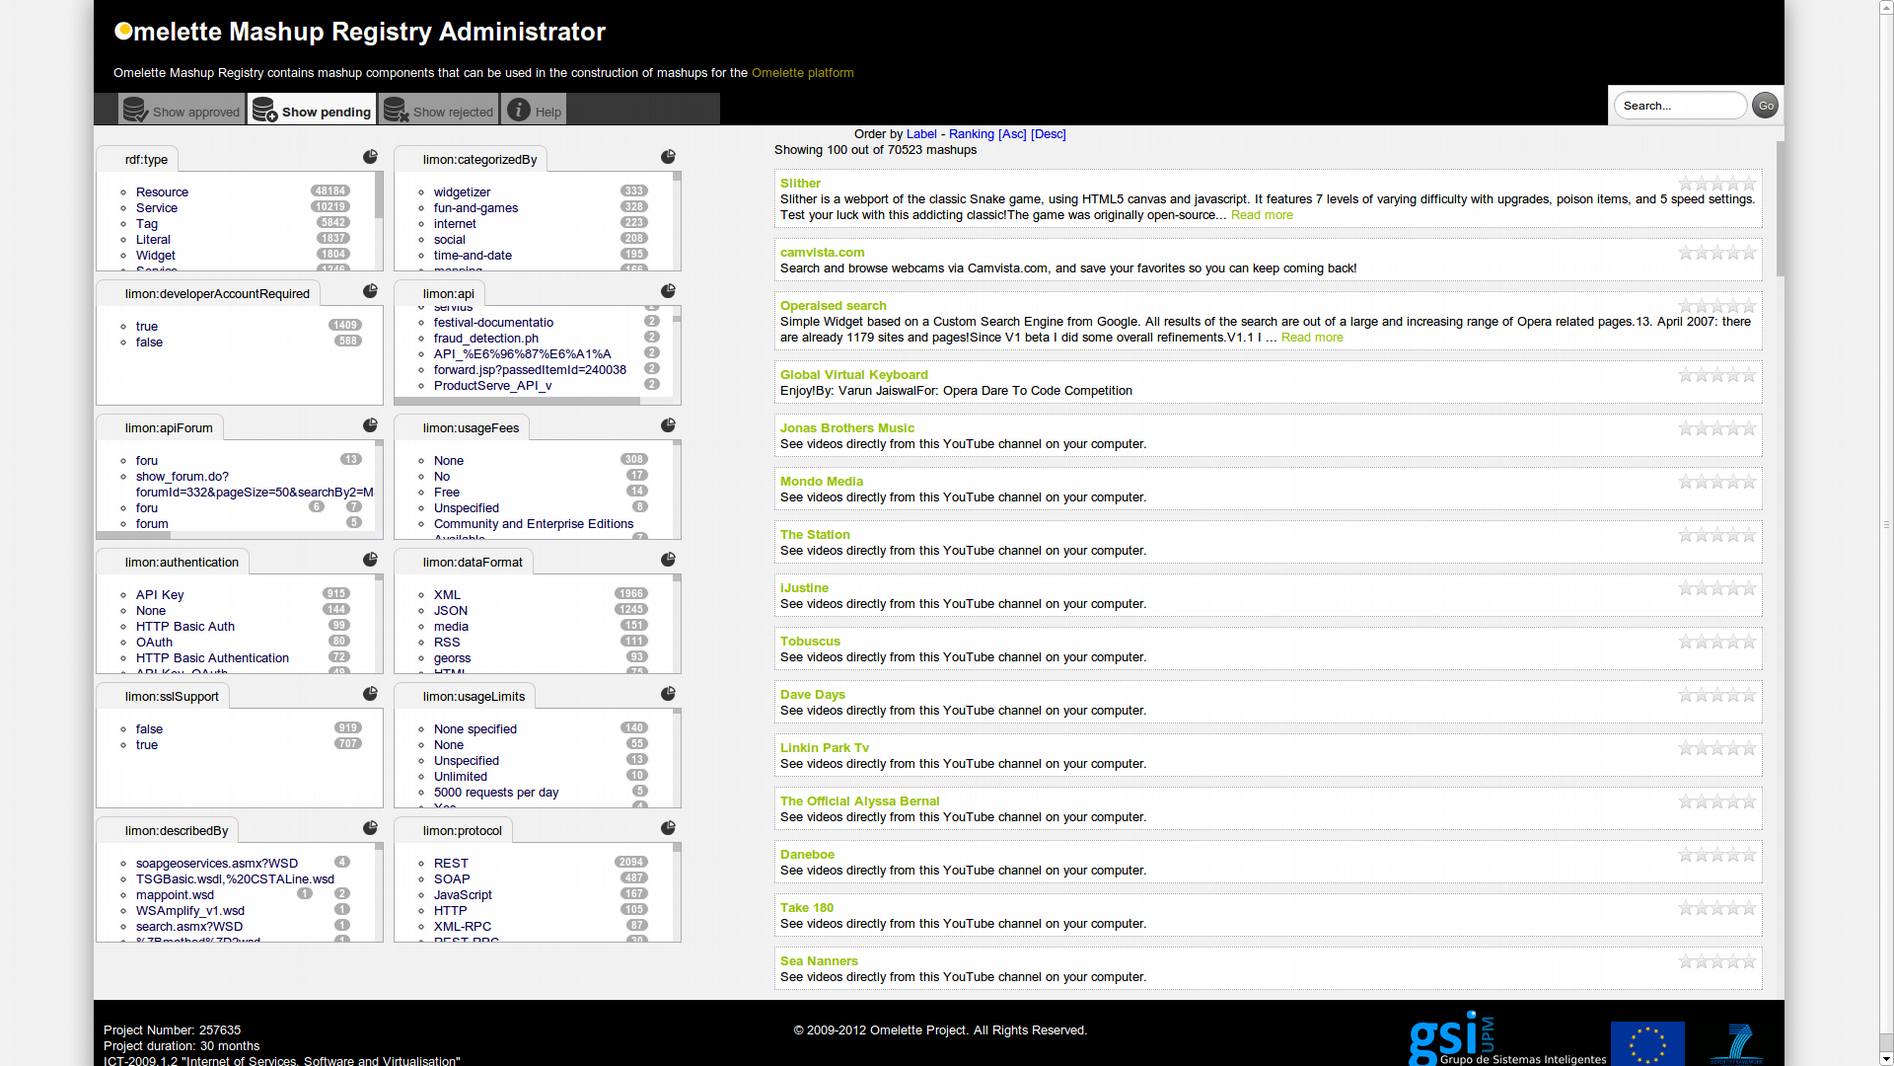
\includegraphics[width=400pt]{graphics/omr-admin-main.png}
%	\caption{Main view OMR Administrator}
%	\label{fig:omradminmainview}
%\end{figure}
%
%\section{OMR admin interface user manual}
%In the main view of the OMR Administrator, a menu is shown at the top:
%
%\begin{figure}[h]
%	\centering
%	
\includegraphics[width=200pt]{graphics/admin-top-menu.png}
%	\caption{OMR admin top menu}
%	\label{fig:topmenuomr}
%\end{figure}
%
%\begin{description}
%\item[Show approved] shows those mash-ups which have been selected by the
%administrator as approved.
%\item[Show pending] shows everything that that has been returned has the output of the
%scrapping process.
%\item[Show rejected] shows the lists of mash-ups that have been previously rejected by
%the administrator.
%\end{description}
%
%\subsection{Show approved content}
%In order to view all approved content, go to “Show approved”.
%
%In the page are shown those mash-ups selected as approved by the administrator in the
%“Show pending” page.
%If no mash-up has been approved before entering here the content would be blank.
%The following actions are available from here:
%\begin{itemize}
%\item Filtering
%\item Searching
%\item Obtaining help
%\item Statistics
%\end{itemize}
%
%\subsection{Show pending content}
%When clicking on the “Show pending” button the screen will be very similar to the others. See figure \ref{fig:admininterfacemain}.
%
%The actions available in the page are:
%\begin{itemize}
%\item Filtering
%\item Searching
%\item Obtaining help
%\item Statistics
%\item Validate content: If there are mashups to mark as approved, the checkbox on the left
%   of its title has to be checked. After this, clicking on “Validate selected” button will mark
%      the content as validated in the database, and it will appear in the “Show approved
%       page”.
%\item Reject content if there are mashups to mark as rejected, the checkbox on the left of
%   its title has to be checked. After this, clicking on “Reject selected” button will mark the
%      content as rejected in the database, and it will appear in the “Show rejected page”.
%\end{itemize}
%
%\subsection{Available general actions}
%Here we described various actions available for all pages in the OMR Admin interface.
%
%\subsubsection{Filtering}
%To filter using the filtering boxes click on a property from a filtering category.
%Many filters can be selected at the same time. First select one of them, the view will refresh
%with the new results. Then select next filter, the former filter will be sill selected, and results
%will be filtered by many filters as chosen.
%
%\subsubsection{Searching}
%You can also use the search box to find something by name or description and the ordering.
%It can also be combined at the same time with Filtering.
%
%\subsubsection{Obtaining help}
%For those titles which are not self explicative, information help is shown in pop-up format
%when the mouse is over them
%
%\begin{figure}[h]
%	\centering
%	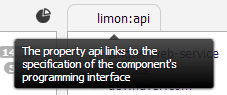
\includegraphics[width=200pt]{graphics/omr-admin-help.png}
%	\caption{OMR admin help}
%	\label{fig:omradminhelp}
%\end{figure}
%
%\subsubsection{Statistics}
%\label{subsec:appendixstatistics}
%
%When large amount of data is presented as in the filtering boxes, it appears an icon which is
%clickable that makes appear a pop-up window showing a graph containing all this information.
%An example is provided in the Figure \ref{fig:omradminseestatistics}
%
%\begin{figure}[h]
%	\centering
%	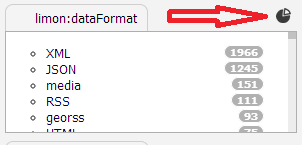
\includegraphics[width=200pt]{graphics/omr-admin-see-statistics.png}
%	\caption{OMR see statistics}
%	\label{fig:omradminseestatistics}
%\end{figure}



